\section{$* \rightarrow \omega$}

\subsection{ language operators}

We already introduced $\lim$. We can define a family of language operators, partly also derived from the study of $\Lang^\omega(reg)$. Some of these operators operate on a single language and not on the class. Let $\Lang$ be a $*$-language class. Let $L \in \Lang$.

\begin{enumerate}
\item $\ext(L) := \Set{\alpha \in \Sigma^\omega}{ \exists n \colon \alpha[0,n] \in L} = L \cdot \Sigma^\omega$
\item $\dext(L) := \Set{\alpha \in \Sigma^\omega}{ \forall n \colon \alpha[0,n] \in L} = L \cdot \Sigma^\omega$
\item $\BC \ext$
\item $\lim(L) := \Set{ \alpha \in \Sigma^\omega }{ \forall N \colon \exists n > N \colon \alpha[0,n] \in L } = \Set{ \alpha \in \Sigma^\omega }{ \exists^\omega n \colon \alpha[0,n] \in L }$
\item $\dlim(L) := \Set{ \alpha \in \Sigma^\omega }{ \exists N \colon \forall n > N \colon \alpha[0,n] \in L }$
\item $\BC \lim$
\item Kleene-Closure of $\Lang$: $\Kleene(\Lang) := \Set{ \bigcup_{i=1}^n U_i \cdot V_i^\omega}{U_i, V_i \in \Lang}$
\item $\Set{\bigcup_{i=1}^n U_i \cdot \lim V_i}{U_i, V_i \in \Lang}$
\end{enumerate}

From language operators, we get language class operators in a canonical way, e.g. $\lim(\Lang) := \Set{\lim L}{L \in \Lang}$.

\subsection{$\Lang^*(reg)$}

Considering $\Lang := \Lang^*(reg)$, we get a language diagram like:

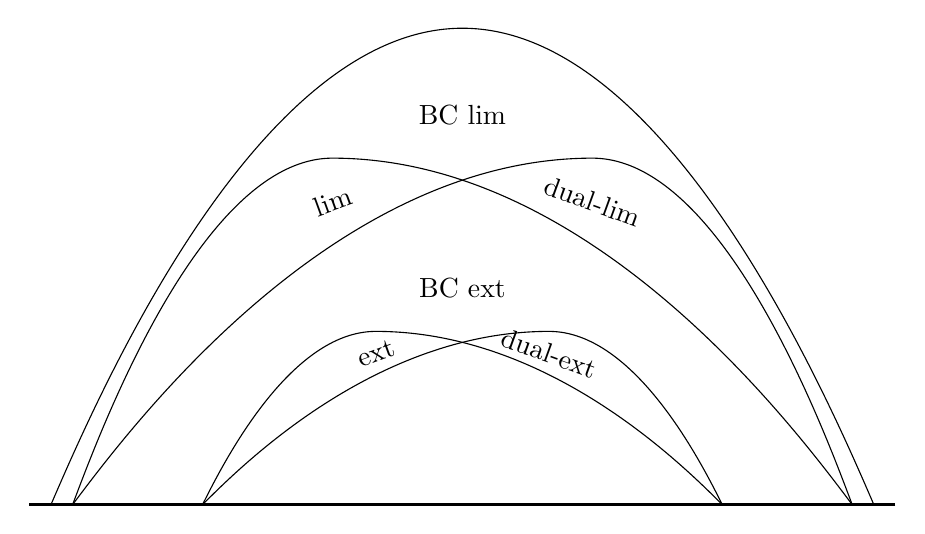
\begin{tikzpicture}
\pgftransformscale{.55}

% http://www.texample.net/tikz/examples/complexity-classes/

%%% HELP LINES - uncomment to design/extend
% \draw[step=1cm,gray,very thin] (-10,0) grid (10,12);
% \node at (0,0) {\textbf{(0,0)}};

%% Horizontal bar
\draw[very thick] (10,0) -- (-10,0);

% BC lim
\draw (-9.5,0) parabola bend (0,11) (9.5,0);
\node at (0,9) {BC lim};

% lim
\draw (-9,0) parabola bend (-3,8) (9,0);
\node[rotate=20] at (-3,7) {lim};

% dual-lim
\draw (-9,0) parabola bend (3,8) (9,0);
\node[rotate=-20] at (3,7) {dual-lim};

% BC ext
%\draw (-6.5,0) parabola bend (0,6) (6.5,0);
\node at (0,5) {BC ext};

% ext
\draw (-6,0) parabola bend (-2,4) (6,0);
\node[rotate=20] at (-2,3.5) {ext};

% dual-ext
\draw (-6,0) parabola bend (2,4) (6,0);
\node[rotate=-20] at (2,3.5) {dual-ext};

\end{tikzpicture}

where all inclusions are strict. In more detail:

% overview of references: S50.1
% S50.2:
\label{P:reg-star}
\begin{itemize}
\item P1: $\ext \Lang \cap \dext \Lang \neq \emptyset$ \newline
Proof: $\tilde{L}_1 := a \Sigma^\omega \in \ext \cap \dext \Lang$ with $\tilde{L}_1 = \ext(a)$ and $\tilde{L}_1 = \dext (a \Sigma^*)$. (R101, prop, p.38)
\item P2a: $\ext \Lang \cap \dext \Lang \subsetneqq \ext \Lang$ \newline
Proof: $\tilde{L}_{2a} := \ext(a^* b) = a^* b \Sigma^\omega \in \ext \Lang$. Assume some A-automaton $\A$ with $n$ states accepts $\tilde{L}_{2a}$. $\A$ would also accept $a^n b^\omega$. I.e. the $(n+1)$th state after the run of $a^n$ would also accept $a$, i.e. $\A$ would accept $a^{n+1}$. By inclusion, $\A$ would accept $a^\omega$. That is a contradiction. Thus, there is no such A-automat. Thus, $\tilde{L}_{2a} \notin \dext \Lang$.
\item P2b: $\ext \Lang \cap \dext \Lang \subsetneqq \dext \Lang$ \newline
Proof: $\tilde{L}_{2b} := - \tilde{L}_{2a} \in \dext \Lang$, $\tilde{L}_{2b} \notin \ext \Lang$.
\item P3: $\ext \Lang \neq \dext \Lang$ \newline
Proof: Follows directly from P2a and P2b.
\item P4: $\ext \Lang \cup \dext \Lang \subsetneqq \BC \ext \Lang$ \newline
Proof: $\tilde{L}_4 := \Sigma^* a \Sigma^\omega \cap -(\Sigma^* b \Sigma^\omega)$, $\Sigma = \Set{a,b,c}$. Then we have $\tilde{L}_4 \notin \ext \cup \dext \Lang$, $\tilde{L}_4 \in \BC \ext \Lang$. (R101, p.38)
\item P5: $\BC \ext \Lang = \lim \Lang \cap \dlim \Lang$ \newline
Proof: \ref{gen:staiger-wagner} (Staiger-Wagner-recognizable)
%S405 / Staigner-Wagner-recognizable
\item P6a: $\lim \Lang \cap \dlim \Lang \subsetneqq \lim \Lang$ \newline
Proof: $\tilde{L}_{6a} := \lim(\Sigma^* a) = (\Sigma^* a)^\omega$. Assume there is $L \subseteq \Sigma^*$ with $\lim(L) = -\tilde{L}_{6a}$. Let $(w_0,w_1,w_2,\dotsc) \in (\Sigma^*)^\N$ so that $w_0 \in L, w_0 a w_1 \in L, \dotsc, w_0 \prod_{i=0}^n a w_i \in L \ \forall n \in \N$. Thus, $\alpha := w_0 \prod_{i \in \N} a w_i \in \lim L$. But $\alpha \notin -\tilde{L}_{6a}$. That is a contradiction. Thus, $-\tilde{L}_{6a} \notin \lim \Lang$. With E3, we get $\tilde{L}_{6a} \notin \dlim \Lang$.
\item P6b: $\lim \Lang \cap \dlim \Lang \subsetneqq \dlim \Lang$ \newline
Proof: Analog to P6a with $\tilde{L}_{6b} := -\tilde{L}_{6a}$.
\item P7: $\lim \Lang \neq \dlim \Lang$ \newline
Proof: Follows directly from P6a and P6b.
\item P8: $\lim \Lang \cup \dlim \Lang \subsetneqq \BC \lim \Lang$ \newline
%(S408, S409)
Proof: $\tilde{L}_8 := (\Sigma^*a)^\omega \cap -(\Sigma*b)^\omega$. Then $\tilde{L}_8 \notin \lim \cup \dlim \Lang$ but $\tilde{L}_8 \in \BC \lim \Lang$. (R101, prop, p.38)
\item P9: $\BC \lim \Lang = \Set{ \bigcup_{i=1}^n U_i \cdot V_i^\omega}{U_i, V_i \in \Lang}$ \newline
%(S402, S407)
Proof: This is explained already in chapter \ref{reg-omega-lang}. 
\item P10: $\BC \lim \Lang = \Set{\bigcup_{i=1}^n U_i \cdot \lim V_i}{U_i, V_i \in \Lang}$ \newline
%(S403, S411) (R107, Theorem 3.1)
Proof: This is explained already in chapter \ref{reg-omega-lang}. 
\item P11: $\BC \lim \Lang = \Set{L_{\text{B"uchi}}^\omega(\A)}{\A \text{ automaton so that } L^*(\A) \in \Lang}$ \newline
Proof: (R101,Th.12,p.9) says $\Set{L_{\text{B"uchi}}^\omega(\A)}{\dots} = \Set{ \bigcup_{i=1}^n U_i \cdot V_i^\omega}{U_i, V_i \in \Lang}$. The rest follows with P9.
\end{itemize}

\subsection{Questions}

This was studied in detail for $\Lang^*(reg)$. We are now studing relations of resulting $\omega$-language classes for different $*$-language classes.

% \stackrel{?}{\le} or \overset{?}{\le}
Esp.:
\begin{itemize}
\item $\BC \ext \Lang \overset{?}{=} \BC \lim \Lang$
\end{itemize}

